\section{System Overview}\label{sec-arch}
In this section, we give an overview of the entire architecture of SVC.
We first define the scope of SVC including which types of views and queries we address.
Then, we briefly present each of the components of our system.

\subsection{Problem Setting}
%In this paper, we only consider insertions to the base table, see
%\reminder{Extended Paper} for more details on how to model deletions.
\vspace{-.5em}
\subsubsection{Materialized Views}
In this paper, we evaluate SVC on three classes of materialized views, Select-Project, Foreign-Key Join, and Aggregation:
\vspace{0.25em}

\noindent\textbf{Select-Project Views (\spview): } These views are defined by Select-Project
expressions of the following form:

\begin{lstlisting}
SELECT [a1,a2,...] FROM Table 
WHERE Condition(A);
\end{lstlisting}

\vspace{0.25em}

\noindent\textbf{Foreign-Key Join Views (\fjview): } As an extension to the Select-Project Views, we can support views derived from a Foreign-Key join:

\begin{lstlisting}
SELECT table1.[a1,a2,...], table2.[a1,a2,...],...
FROM Table1, Table2,...
WHERE Table1.fk = Table2.fk AND Condition(A);
\end{lstlisting}

\vspace{0.25em}

\noindent\textbf{Aggregation Views (\aggview): } We also consider views defined by group-by aggregation queries of the following form:

\begin{lstlisting}
SELECT [f1(a1),f2(a2),...] 
FROM Table 
WHERE Condition(A)
GROUP BY [a3,a4,...];
\end{lstlisting}

\vspace{0.25em}

We selected these classes of views to be specific enough to analyze in terms of cost but general enough to evaluate using real datasets and query workloads.
%There are, however, other types of materialized views that SVC can support including views defined by aggregate queries with \havingfunc clauses.

\subsubsection{Updates}
There are three types of updates that can affect a base table: \insertion, \delete, \update.
Insertion-only workloads are increasing common \cite{grund2009vertical} in enterprise applications.
Thus, the primary focus of this paper is on analysis and results for \insertion. 
In Section \ref{sec:del}, we discuss how to modify our query processing to support \delete, which in turn allows us to support \update.
We can model \update as a \delete of the old record then an \insertion of a new record with updated values. 

\subsubsection{Supported Queries} \label{subsubsec:queries}
In this paper, we focus on answering three commonly used aggregation queries on the view.
For ease of presentation, we assume the query does not have a group-by clause, which can be easily extended by treating each group key as an additional condition of the query: 
\begin{lstlisting} [mathescape]
SELECT $\sumfunc(a)/\countfunc(a)/\avgfunc(a)$ FROM View 
WHERE Condition(A);
\end{lstlisting}
For these queries, we prove optimality of our approach with respect to estimate variance (Section \ref{subsec:correct-practical}). 
We also provide support for correcting stale Select queries of the following form:
\begin{lstlisting} [mathescape]
SELECT * FROM View 
WHERE Condition(A);
\end{lstlisting}
Since the results of these queries are not numeric, we instead bound the cardinality of the results.
Refer to Section \ref{sec:sel} for a discussion of how to correct Select queries with SVC. 

%\subsubsection{Supported Materialized Views}\label{subsubsec:supported-view}
%We will first introduce the taxonomy of materialized views that can benefit from our approach. 
%In this paper, we analyze and experiment with three classes of views: Select-Project Views, Foreign-key Join Views, and Aggregation Views.
%Our technique can be applied to a broader class of views, please refer to [?] for a full description.


%There is a taxonomy of aggregation views and we discuss different types of aggregate functions (distributive, algebraic, holistic) can be applied in our framework \reminder{Extended Paper}.



%Modeling incremental maintenance as a data cleaning problem gives as a new perspective.
%Staleness in a materialized view row is a type of data error.
%A row 

%When rows in the materialized view are stale

%Frequent incremental maintenance of materialized views can be challenging given system resource constraints.
%Existing materialized view maintenance techniques lie on a spectrum of freshness and performance.
%Immediate maintenance guarantees that query results on the view will always be fresh, while batch maintenance allows for a higher throughput of updates to the base table.
%These two techniques sit at the extremes of the spectrum since they still require that all updates are processed and propagated to the view.



%Thus, our results are never stale; \reminder{This claim is a little strong. Since we do batch job, is it also possible for us to give stale results?} they have some inaccuracy introduced by the sampling ratio but in expectation they are correct.
%Furthermore, we also prove that this correction term is the optimal linear unbiased estimate for SUM, COUNT, and AVG.

\subsection{System Architecture}
Modeling view maintenance as a data cleaning problem gives us a new perspective for addressing staleness.
Insertions to the base table can cause two types of errors in the view: rows are either out-of-date or missing altogether.
The challenge is to ``clean" the materialized view by updating the out-of-date rows and inserting the missing rows, however this can be very expensive if there are a large number of new records to process.
Cleaning a sample of dirty rows potentially reduces the amount of updates, join executions, and aggregates we need to compute.
From this sample, we can derive a correction to stale query results.

The architecture of SVC is shown in the introduction (Figure \ref{sys-arch}).
The diagram depicts the following three components: (1) we sample the ``update pattern",
(2) we use the sample to correct stale queries, and (3) we maintain an index of outliers.

In implementation, SVC will work in conjunction with existing maintenance or re-calculation approaches.
We envision the scenario where materialized views are being refreshed periodically, for example nightly.
While maintaining the entire view throughout the day may be infeasible, sampling allows the database to scale the cost with the performance and resource constraints during the day.
Then, between maintenance periods, we can provide approximately up-to-date query results for aggregation queries.

\subsubsection{Sampling the Update Pattern}
%Given these materialized views, the first challenge is sampling.
The three classes of views require different sampling techniques since they are affected by updates differently.
For example, insertions to the base table only result in insertions to \spview and \fjview.
But, for \aggview, insertions to the base table can also result in updates to existing stale rows.
In Section \ref{sampling}, we describe the sampling techniques and a cost analysis of how much sampling can reduce maintenance costs.

\subsubsection{Correcting a Query}
We can use udpate information from the sample to correct stale query results.
For the aggregate functions, \sumfunc, \countfunc, and \avgfunc, we calculate a correction
which is bounded and provably optimal.
Like the sampling, the algorithm to calculate the correction varies between the types of views.
We detail query correction in Section \ref{correction}.

\subsubsection{Outlier Indexing}
Furthermore, we use an outlier index to reduce the sensitivity of our correction estimates to skewed distributions. 
We guarantee that records (or rows in the view derived from those records) 
in the outlier index are also included in the sample.
This can be used to reduce variance in our estimates.
See Section \ref{outlier} for details on this component.

\subsubsection{Example Application: Log Analysis}
To illustrate our system, we use the following running example which is a 
simplified schema of one of our experimental datasets (Figure~\ref{example-1}).
Imagine, we are querying logs from a video streaming company. 
These logs record visits from users as they happen and grow over time.
We have two tables, \tbl{Log} and \tbl{Video}, with the following schema:

\begin{lstlisting}[mathescape]
Log(sessionId$\textrm{,}$ videoId$\textrm{,}$ responseTime$\textrm{,}$ userAgent)
Video(videoId$\textrm{,}$ title$\textrm{,}$ duration)
\end{lstlisting}
These tables are related with a foreign-key relationship between
Log and Video, and there is an integrity constraint that every log
record must link to one video in the Video table.

\begin{figure}[ht!] 
\centering
\vspace{-0.75em}
 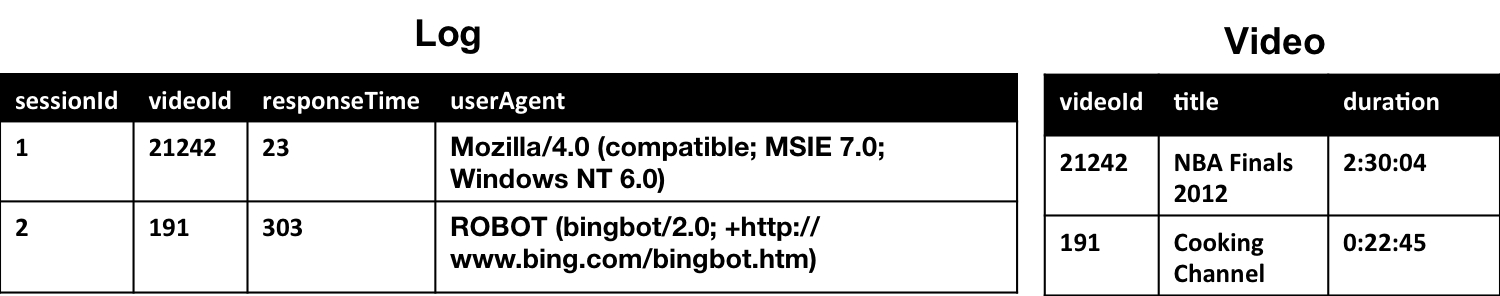
\includegraphics[width=\columnwidth]{figs/sample-clean-example.png}\vspace{-0.25em}
 \caption{A simplified log analysis example dataset. In this dataset, there are two tables: a fact table representing video views and a dimension table representing the videos.\label{example-1}}
\end{figure}

Consider the following example materialized view \aggview, which stores a result for each video and the maximum time it took for the server to load that video:
\begin{lstlisting} 
SELECT videoId, 
max(responseTime) AS maxResponseTime 
FROM Log 
GROUP BY videoId;
\end{lstlisting}

The user wants to know how many videos had a max response time of greater than 100ms.
\begin{lstlisting} 
SELECT COUNT(1)
FROM AggView
WHERE maxResponseTime > 100;
\end{lstlisting}
Let us suppose the initial query result is $45$.
There now have been new log records inserted into the Log table making the old result stale.
For example, if our sampling ratio is 5\%, that means for 5\% of the videos (distinct videoID's) we refresh stale maxResponseTime if necessary.
From this sample, we calculate how many new videos changed from a maxResponseTime of less than 100ms to times greater than 100ms; let us suppose this answer is $2$.
Since our sampling ratio is 5\%, we extrapolate that $40$ new videos throughout the view should now be included in the count.
This means that we should correct the old result by $40$ resulting in the estimate of $85$.
In contrast, if we had applied SAQP, we would have counted how many videos in the sample had a max response time of greater than 100ms.